%!TEX root = proyecto.tex

\chapter{Introducción}

\lettrine[lines=4]{L}{a} visión artificial  es un ámbito de la informática que surgió hace 60 años, centrado en el estudio del procesamiento digital de las imágenes. En los últimos años ha tomado mucha importancia el reconocimiento facial, problema consistente en identificar rostros humanos dentro de una imagen,  gracias a la investigación realizada por \textit{Viola y Jones} en 2001, y la reciente tendencia en \textit{smartphones} con el desbloqueo facial. 
\vspace*{-5mm}
\section{Historia de la Visión Artificial}
\vspace*{-5mm}
Uno de los primeros acontecimientos que propició la visión artificial fue la creación del cable Bartlane, capaz de transmitir una imagen a través del océano Atlántico en los años 1920, con una duración de cerca a una semana \cite{gonzalez_woods_2018}. Pero, dentro del entorno del procesamiento de imágenes digitales, la investigación se centró en recuperar una estructura tridimensional del mundo real a través de una imagen, para conseguir un entendimiento total de la escena que plasma la misma. Debido a esto, aparecieron varios algoritmos de reconocimiento de líneas, donde uno de ellos fue creado por parte de Huffman en 1971 \cite{szeliski_2018}.

Uno de los descubrimientos que inició este movimiento no fue proveniente de la informática, sino de la psicología. Esta sería una de las principales fuentes sobre el entendimiento de cómo funciona la visión.  Un par de psicólogos, David Hubel y Torsten Wiesel, describieron que el comportamiento de las neuronas encargadas de entender el entorno visual siempre empieza con estructuras simples como vértices. Más tarde, esta idea se convertirá en el principio central del \textit{Deep Learning}.

Russell Kirsch, en 1959, es el primero en desarrollar un aparato que traducía las imágenes en datos que las máquinas pudiesen entender. Y, Lawrence Roberts en 1963 publica un estudio sobre cómo las máquinas pueden percibir objetos sólidos de tres dimensiones \cite{histComputer}, uno de los avances considerados precursores de la visión artificial moderna.

Durante los años 1980, se desarrolló una red artificial capaz de reconocer patrones, mediante el uso de una red convolucional, que propició la creación de un modelo llamado LeNet-5, la primera red convolucional moderna. Este modelo se caracteriza por usar la \textit{backpropagation} \cite{histComputer}. Mientras que en los años 1990 la visión artificial cambia totalmente de rumbo y los investigadores pasaron de intentar reconstruir objetos en 3D a intentar detectar objetos mediante sus características.

A partir del año 2000 se hacen muchos avances importantes y que actualmente son usados en aplicaciones reales. El primer detector facial llegaría en 2001, creado por Paul Viola y Michael Jones \cite{paulViola}. Ambos consiguieron crear el primero que funcionaba en tiempo real.

El problema de estos modelos es el uso de información para poder entrenarlos. Como consecuencia, se creó un proyecto llamado PASCAL VOC, que creó un dataset estándar para la clasificación de objetos \cite{pascalVOC}. Posteriormente, apareció en 2010 ImageNet, el cual contiene más de un millón de imágenes para un total de mil objetos. Junto a este apareció un modelo basado en una red convolucional llamado AlexNet \cite{krizhevsky2014weird}. Desde entonces, el \textit{Deep Learning} se ha convertido en eje central del avance en la visión artificial, conjuntamente con todos los avances matemáticos realizados anteriormente.
\vspace*{-10mm}
\section{Reconocimiento Facial y COVID-19}

En la actualidad, la visión artificial se utiliza en muchos proyectos y está presente en investigaciones muy importantes para el futuro de la inteligencia artificial. Una de ellas se basa en el reconocimiento facial, y es usado en aplicaciones para reconocer personas, gestos, atributos faciales, contar las personas, etc. 

La detección facial se inicia con una imagen arbitraria, con el objetivo de encontrar todas las caras que hay en ella, y posteriormente devolver la localización exacta de cada una de las caras. Aunque esta tarea es natural para los humanos, es bastante complicada para los ordenadores, ya que se encuentran muchos factores que lo dificultan, tales como: la escala, localización, punto de vista, iluminación, lentes, etc. Existen centenares de investigaciones/proyectos sobre detección facial, desde uno de los más influyentes en los años 2000, como \textit{Viola and Jones face detection}, a proyectos basados en \textit{Deep Learning}, con tecnologías como \textit{Tensorflow} o \textit{YOLO} \cite{szeliski_2018}. 

Tras el año 2020 y la aparición del COVID-19, el uso de mascarillas y el cumplimiento de las normas impuestas por la OMS (Organización Mundial de la Salud) están al orden del día. En este trabajo se tendrá como objetivo el estudio de todas estas tecnologías para poder controlar el uso correcto de la mascarilla facial, terminando con un prototipo capaz de detectar cuando una personas lleva mascarilla. En la Figura \ref{fig:2} se puede ver un ejemplo del uso correcto, incorrecto y mal uso de la mascarilla, extraído del dataset de caras usado en la experimentación.

\begin{figure}[htp]
	\centering
	\begin{subfigure}{0.2\linewidth}
		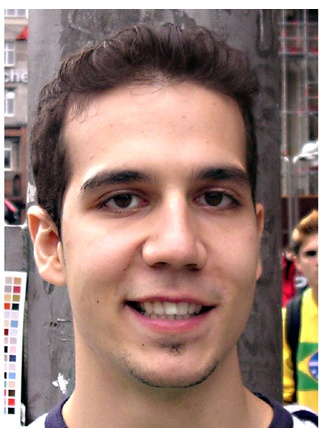
\includegraphics[width=\linewidth]{imagenes/dataset2-1.jpg} 
		\caption{}
		\label{fig:2a}
	\end{subfigure}\hfill
	\begin{subfigure}{0.4\linewidth}
		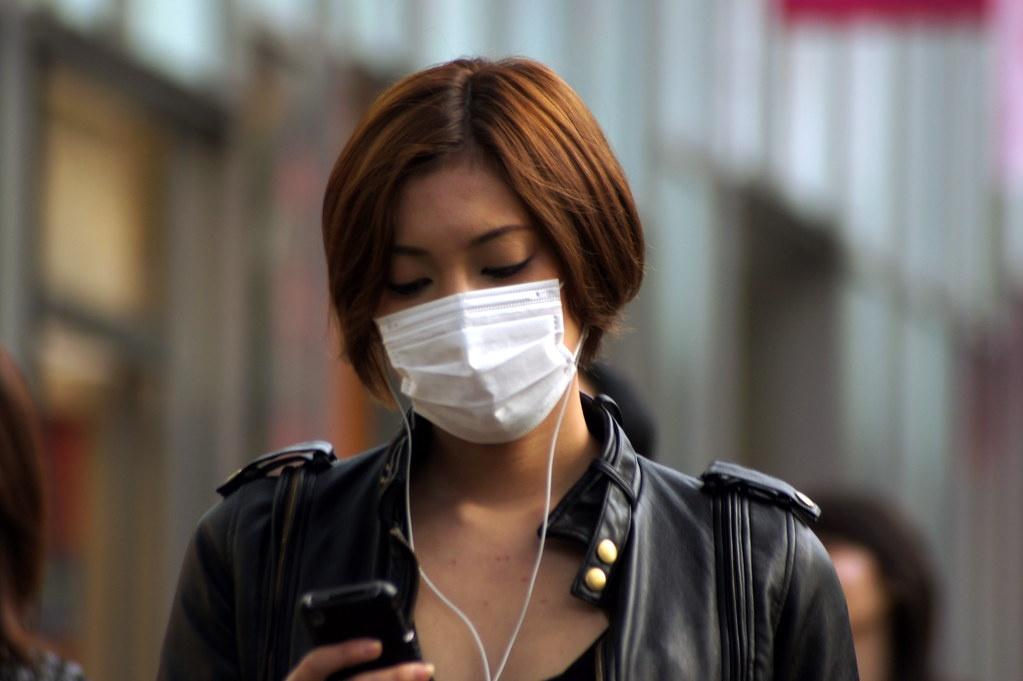
\includegraphics[width=\linewidth]{imagenes/dataset2-2.jpg}
		\caption{}
		\label{fig:2b}
	\end{subfigure}\hfill	
	\begin{subfigure}{0.3\linewidth}
		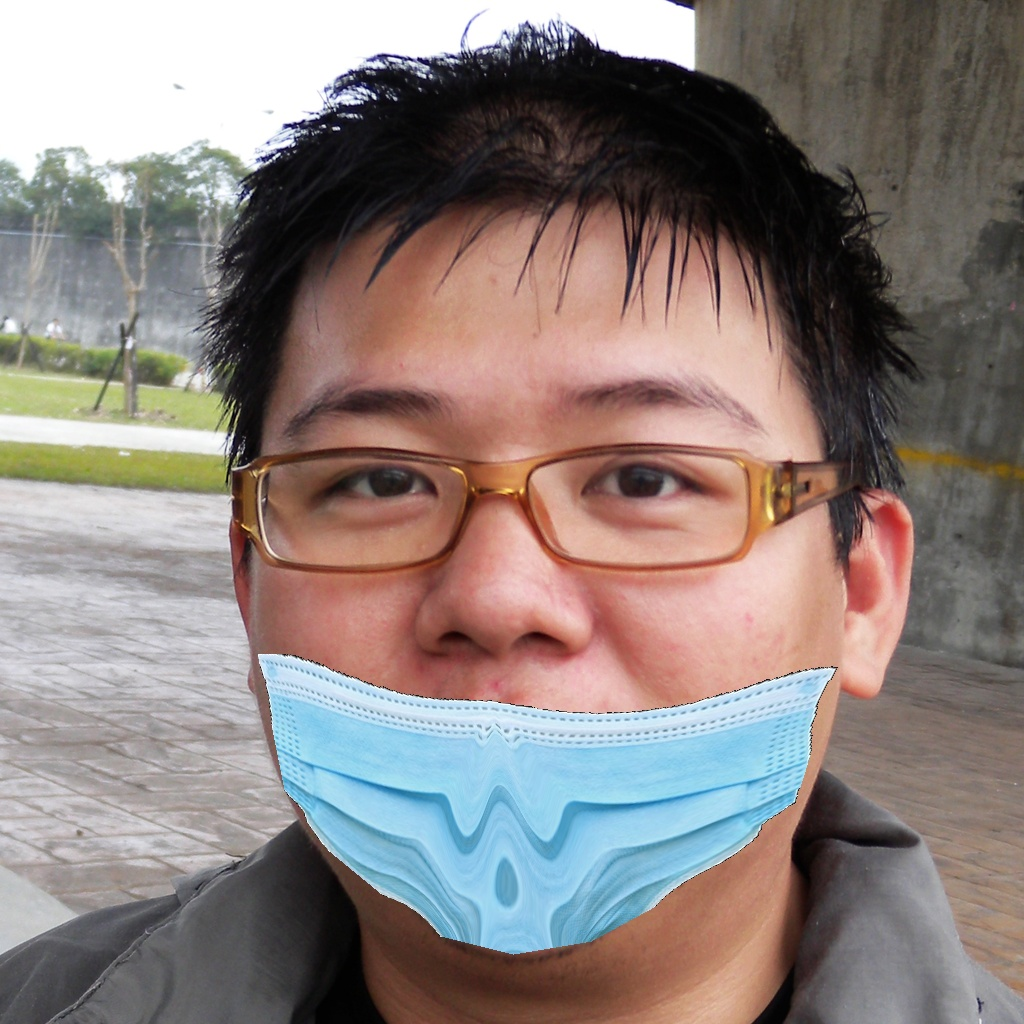
\includegraphics[width=\linewidth]{imagenes/dataset2-3.jpg}
		\caption{}
		\label{fig:2c}
	\end{subfigure}
	\caption[Ejemplos del uso de la mascarilla]{Ejemplos del uso de la mascarilla, extraídos del dataset usado en la experimentación.}
	\label{fig:2}
\end{figure}

La creación de un prototipo capaz de realizar esta comprobación permitiría su uso en la entradas a locales, comercios, transporte público, festivales, etc. Ofreciendo la posibilidad de la creación de aplicaciones con el uso de este, por ejemplo, la implementación de una aplicación capaz de reconocer si la persona no lleva de forma correcta la mascarilla y tiene fiebre, mediante un detector de temperatura, provocando un aviso.
